% بد نیست که جلسه دفاع، با یک نقل قول مناسب، از یکی از بزرگان شروع شود. این به جلسه شما، حال‌و‌هوای علمی‌ می‌دهد. چون گزارش من، حدودا در شاخه مهندسی نرم‌افزار قرار می‌گرفت از یکی از سخنان آقای <<کیپرز جونز>> استفاده کردم. میشه از سایت‌هایی مثل: https://www.inspiringquotes.us ، http://www.azquotes.com/ یا https://www.brainyquote.com/ نیز استفاده کرد.

\label{quote}
\subsection{در آغاز}

\begin{frame}
\frametitle{در آغاز}

\pause
\begin{columns}[c]
\column{.45\textwidth} % Left column and image
\justify \lr{\lin\fontsize{11}{13.2}\selectfont{"High-quality software is not expensive. High-quality software is faster and cheaper to build and maintain than low-quality software, from initial development all the way through total cost of ownership."}}
\flushright{\lr{\citep{Jones:2011:ESQ:2025240}}} 

\column{.52\textwidth} % Right column and quote
\begin{figure}
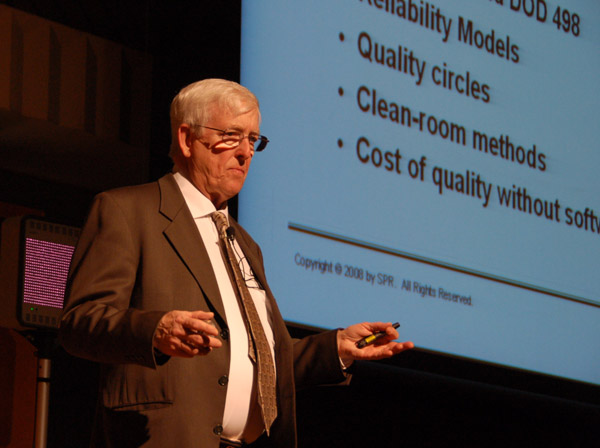
\includegraphics[scale=.3]{resources/img/capers-jones-001.jpg}
\end{figure}
\bigskip
\end{columns}

\end{frame}
